\documentclass[a4paper, norsk, 11pt]{article}
\usepackage[T1]{fontenc} 			% N�dvendig for fonter
\usepackage[latin1]{inputenc} % N�dvendig for ���
\usepackage{babel}						% N�dvendig for dokument
\usepackage{graphicx}					% For � kunne inkludere grafikk
\usepackage{amsmath, amsfonts, amssymb} % Pakker for � skrive matte
\usepackage[amssymb]{SIunits} % For � bruke \unit til SI-enheter


% Tegninger, som b�ndgap
\usepackage{tikz,tkz-tab}
\usetikzlibrary{decorations.pathmorphing}
\usetikzlibrary{shapes,arrows}
\usepackage{xcolor} % Farger
\usepackage{rotating} % Rotere p� stash

\usepackage{hyperref} % For linker til kapitler

\author{Jon Skarpeteig}
\title{Basis dokument}
\date{\today}

\begin{document}
\maketitle

%\section{Introduksjon}

%%INCOMPLETE - mangler masse + stash er feil

Solceller er antatt � dominere energisektoren de neste hundre �r. For at dette skal bli tilfelle trengs det billige og effektive solceller. Multikrystallinsk silisium er materialet som har mest potensiale for � oppn� dette. Det er billig � produsere, men har ogs� relativt lav utnyttelse av solenergien. Derfor er det viktig � n�yaktig kunne identifisere kilder til tap, og forst� virkem�ten til slike materialer. 

Det er oppdrettet et laboratorium for � kunne gj�re m�linger p� slike celler ved hjelp av fotoluminisens p� ekstremt lave temperaturer. Tidligere m�linger av multikrystallinsk silisium p� dette laboratoriet viser deler av et spekter som er � finne p� tilsvarende m�linger (f.eks \cite{tarasov00}), men deler av tapsspekteret som var forventet dukket ikke opp. Dette prosjektet fokuserer p� hva som er �rsaken til dette avviket, og hvordan det kan utbedres. I tillegg til det er det fokusert p� virkem�te til solceller, og kilder til tap i multikrystallinsk silisium.
\section{Solcelle teori}

%TEORIDEL - Solceller - virkem�te, karakteristikker, MC vs. Thinfilm, utforming, 

De fleste solceller er krystallinske, det betyr at strukturen er ordnet, eller periodisk. I praksis vil krystallene inneholde feil av forskjellige slag. Noen solcellematerialer er ikke krystallinske, men mangler langtrekkende periodisitet. Disse best�r da av amorfe materialer.

Et fritt elektron i vakuum vil kunne innta en hvilken som helst energi. Et elektron i en krystallstruktur er bundet av energib�nd atskilt av gap med energitilstander som elektronene ikke kan ha. Det er derfor bare plass til et endelig antall elektroner i hvert b�nd, fordi hver tilstand bare kan romme to elektroner i f�lge Pauli-Prinsippet. For en krystall kan energib�ndene oppfattes som overlapp av enkelttilstander for hvert atom. En kan oppfatte energib�ndene som krystallens 'elektronskall'. 

\begin{figure}[!h]
 \centering
 	% Tegning
 	\begin{tikzpicture}[scale=0.5]
     	\draw[very thick,->] (1,6) -- node[below] {x}  (25,6); % X akse
    	\draw[very thick,->] (1,6) -- node[left] {\begin{sideways}Energi\end{sideways}} (1,18); % Y akse
    
    \begin{scope} % Valens og ledningsb�nd
		    \draw[thick,fill=black!10] (2,7) rectangle node {Valensb�nd} ++(22,4);
        \draw[thick,fill=black!10] (2,13) rectangle node {Ledningsb�nd} ++(22,4);
        \draw[thick,<->] (13,13) -- node[right] {B�ndgap} (13,11); % Pil
    \end{scope}
    \end{tikzpicture}    \caption{Energib�nd}
    \label{fig:energiband}
\end{figure}

Det �verste b�ndet kalles ledningsb�ndet. Energib�ndet umiddelbart under ledningsb�ndet, kalles valensb�ndet. De ikke tillatte tilstandene mellom valensb�ndet og ledningsb�ndet kalles b�ndgapet. Dette b�ndgapet er veldig viktig i forbindelse med solceller og oppgis ofte i elektronvolt (eV). % Legg til kr�llstash p� figur

For at elektronet skal kunne flytte p� seg m� det befinne seg i ledningsb�ndet. Et elektron m� ha nok energi til � kunne eksiteres fra valensb�ndet. Eksitasjon vil si at et elektron forflytter seg fra valensb�ndet til ledningsb�ndet. Dette kan skje ved at elektronet f�r h�y nok energi til � forflytte seg over b�ndgapet ved termisk energi, eller annen energi tilf�rt utenfra, som fra lys. Dette gir �kt ledningsevne til materialet. Samtidig blir det en ledig plass i valensb�ndet, som gj�r at andre elektroner i valsensb�ndet kan f� h�yere kinetisk energi p� grunn av f�rre kollisjoner. Dette p�virker ogs� materialet slik at det f�r h�yere ledningsevne.

Materialer deles ofte inn i tre kategorier; Isolatorer, halvledere, og metaller. Isolatorer har ingen, eller f� elektroner i ledningsb�ndet, som gir dem d�rlig ledningsevne. Metaller har som regel fylte ledningsb�nd ved romtemperatur, som gir dem god ledningsevne. Selv ved 0K har metaller et delvis fylt ledningsb�nd. Halvledere har d�rligere ledningsevne enn metaller, og vil ved 0K ikke ha noen elektroner i ledningsb�ndet. B�ndgapet til halvledere ligger mellom det for isolatorer og metaller, slik at ved romtemperatur er ledningsb�ndet delvis fylt, i motsetning til isolatorer.

\begin{figure}[!h]
 \centering
 % Tegning
 

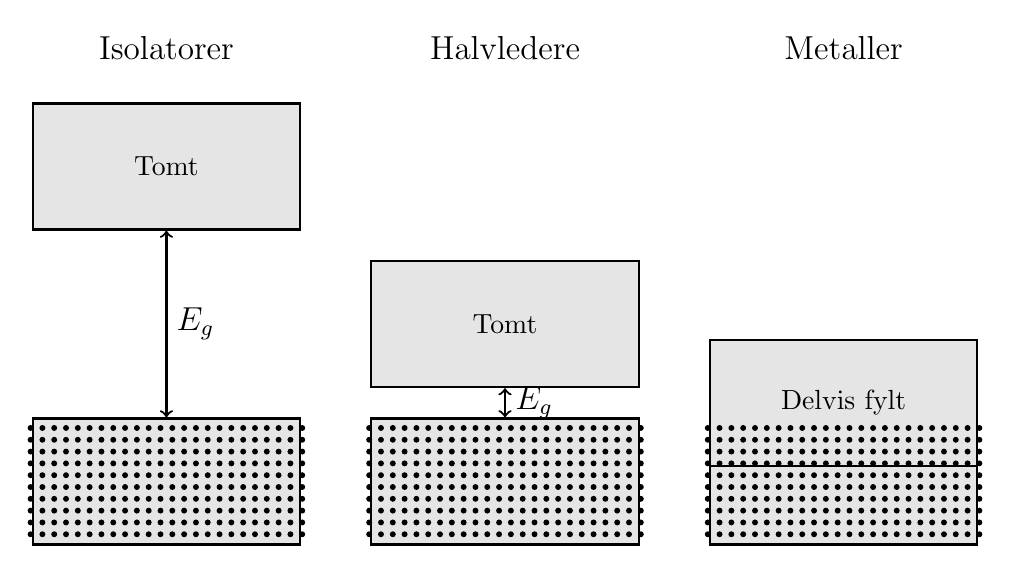
\begin{tikzpicture}
 	% Styles til elementer (kan ogs� v�re generelle utenfor tikzpicture)
	\tikzstyle{ledningsband} 	=	[rectangle, draw, thick, fill=black!10, text width=9em, text centered, minimum height=1.6cm]
	\tikzstyle{valensband}		= [rectangle, draw, thick, fill=black!10, text width=9em, text centered, minimum height=1.6cm]


	% Boksene i bunnen
	\node[valensband]	(valens_isolator)																										{};
	\node[valensband]	(valens_halvleder)	[right of=valens_isolator,  node distance=4.3cm]	{};
	\node[valensband]	(valens_metall)			[right of=valens_halvleder, node distance=4.3cm]	{};	
	
	% Boksene i toppen
	\node[ledningsband]	(lednings_isolator)		[above of=valens_isolator, 	node distance=4cm]	{Tomt};
	\node[ledningsband]	(lednings_halvleder)	[above of=valens_halvleder, node distance=2cm]	{Tomt};
	\node[ledningsband]	(lednings_metall)			[above of=valens_metall, 		node distance=1cm]	{Delvis fylt};
	
	% Piler
	\draw[thick,<->] (valens_isolator)  -- node[right] {\large $E_g$} (lednings_isolator);
	\draw[thick,<->] (valens_halvleder) -- node[right] {\large $E_g$} (lednings_halvleder);
	
	% Tekst p� toppen
	\node (isolator_tekst)  [above of=lednings_isolator,node distance=1.5cm]	{\large Isolatorer};
	\node (halvleder_tekst) [right of=isolator_tekst, 	node distance=4.3cm] 		{\large Halvledere};
	\node (metaller_tekst)  [right of=halvleder_tekst, 	node distance=4.3cm] 		{\large Metaller};
	
	% Elektroner i valensb�nd
	\foreach \y in {0,0.15,...,1.4}
		\foreach \x in {0,0.15,...,3.5} {
			\draw (\x-1.725,\y-0.67) circle (0.03cm) [fill=black];	% Isolator
			\draw (\x+2.575,\y-0.67) circle (0.03cm) [fill=black];	% Halvleder
			\draw (\x+6.875,\y-0.67) circle (0.03cm) [fill=black];	% Metall
		}	
	
\end{tikzpicture}

	    \caption{Typiske b�ndgap ved 0K} 
 \label{fig:bandgap}
\end{figure}
\vspace{30mm}

Typisk b�ndgap for halvleder silisium er 1.1eV, sammenlignet med 5eV for diamant som er en isolator. ~\cite[Kapittel 3]{streetman}

Hull er en beskrivelse for frav�r av elektroner i valensb�ndet. Et hull vil oppst� n�r et elektron eksiteres fra valensb�ndet til ledningsb�ndet. Lite b�ndgap, og h�y temperatur vil gi vesentlig flere elektroner i ledningsb�ndet, enn for lave temperaturer og stort b�ndgap. Dette beskrives med massevirkningsloven:

\begin{equation}
np=N_cN_ve^{-\frac{E_g}{kT}}
\label{eq:massevirkningsloven}
\end{equation}

der $n$ er antall elektroner, $p$ er antall hull, $N_c$ og $N_v$ er konstanter for gitte materialer. $E_g$ er b�ndgapet, $k$ er Boltzmanns konstant og $T$ er temperaturen i Kelvin. For en intrinsikk halvleder, det vil si en halvleder uten noe form for doping, for eksempel ren silisium, kan massevirkningsloven skrives:

\begin{equation}
np=n_i^2
\label{eq:massevirkningsloven_intrinsikk}
\end{equation}

der 

\begin{equation}
n_i=\sqrt{N_c N_v}e^{-\frac{E_g}{2kT}}
\label{eq:intrinsikk}
\end{equation}

Fra massevirkningsloven kommer det av $E_g$ er en avgj�rende faktor for om en krystall kan sies � v�re en halvleder eller ikke. 


\subsection{Doping}

Ved � sette inn andre atomer i en krystallstruktur, med en annerledes elektronfordeling er det mulig � �ke elektroner i ledningsb�ndet uten � endre konsentrasjonen av hull i valensb�ndet. Dette kalles donor-doping. Et eksempel p� donor-doping er � tilsette fosfor i en silisiumkrystall. Dette vil f�re til flere elektroner i ledningsb�ndet, da fosfor har et valenselektron mer enn silisium og valensb�ndet er tiln�rmet fullt. Fosfor vil i dette tilfellet kalles donor i denne donor-dopingen. Doping konsentrasjonen er vanligvis s� liten at b�ndstrukturen ikke forstyrres vesentlig. Hvis en for eksempel setter inn bor istedenfor fosfor, vil silisium krystallen bli akseptor-dopet. Bor har et mindre elektron i valensb�ndet enn silisium, og vil derfor tilf�re et hull ekstra i valensb�ndet. Som regel er donorkonsentrasjonen av hull og elektroner i henholdsvis valens- og ledningsb�nd vesentlig h�yere enn den intrinsikke, slik at det er en god tiln�rming � sette

\begin{equation}
n \approx N_d
\label{eq:donordoping}
\end{equation}

for donordoping, og

\begin{equation}
n \approx N_a
\label{eq:akseptordoping}
\end{equation}

for akspetordoping. Der $N_d$ er donorkonsentrasjonen, og $N_a$ er akseptorkonsentrasjonen.

En dopet halvleder omtales generelt som ekstrinsikk. Hvis en halvleder er dopet med overtall av donor atomer, har den overtall av elektroner, og kalles n-dopet. For akseptordoping omtales halvlederen som p-dopet, da den har overtall av hull. Den dominerende ladningsb�rertypen kalles for majoritetsb�reren. Majoritetsb�rerene vil v�re de som i hovedsak s�rger for str�mtransporten gjennom halvlederen.


\subsection{Transport- og rekombinasjons-prosesser}

Det er to mekanismer som bidrar til transport av elektroner og hull i halvledere: drift og diffusjon. Drift er transport av en ladd partikkel p� grunn av et elektrisk felt. For transport av et hull i en dimensjon er str�mmen $I_p$ lik antall hull $N_p$ ganger ladning $q$ som krysser et tverrsnitt.

\begin{equation}
I_p = N_p q
\label{eq:diffusjonsstrom}
\end{equation}

I vakuum vil et elektrisk felt akselerere hullene, og hastigheten vil stadig �ke. I halvledere vil det oppst� kollisjoner med atomene i halvlederen, som gir hullene en midlere hastighet s� lenge feltet er konstant. Denne midlere driftshastigheten er relatert til feltet via hullenes mobilitet $�_p$

\begin{equation}
v_p = �_p E
\label{eq:elektronfart}
\end{equation}

Hvis alle hullene beveger seg i samme retning kan en da beregne str�m per areal, eller str�mtetthet.

\begin{equation}
J_p = \frac{I_p}{A} = \frac{N_p q}{A} = pAv_p \frac{q}{A} = pv_p q = pq�_p E
\label{eq:hulltetthet}
\end{equation}

Kombinert med tilsvarende uttrykk for elektroner:

\begin{equation}
J = J_p + J_n = (nq�_n + pq�_p)E = \sigma E
\label{eq:stromtetthet}
\end{equation}

der $�_n$ er mobiliteten for elektroner, og $\sigma$ er halvlederens ledningsevne. $J_n$ er elektronstr�mtettheten.

Str�mmen blir da 

\begin{equation}
I = JA = A\sigma E = \left( \frac{A\sigma}{L}\right)V
\label{eq:strom}
\end{equation}

Halvledere vil typisk ha ledningsevne $10^{-8}$ til $10^3$ S\per\metre. Typiske verdien for isolatorer og metaller er henholdsvis $10^{-14}$ og $10^6$ S\per\metre ~\cite[Kapittel 4]{streetman}


%%%%%%%%%%% title?

Elektronet kan g� fra det ene b�ndet til det andre direkte eller indirekte. Ved indirekte generasjon og rekombinasjon kan elektronet benytte seg av s�kalte gap-tilstander. Dette er tilstander somer knyttet til forurensinger, defekter i krystallstrukturen, grenseflater mellom krystallkorn for multikrystallinske materialer, og overflater. Gap-tilstander ligger mellom valensb�ndet og ledningsb�ndet, som er ikke tillatte tilstander for en perfekt krystal (se fig. \ref{fig:indirekte})\\


\begin{figure}[!h]

\begin{tikzpicture}

% Styles til elementer
\tikzstyle{band} 	=	[rectangle, draw, thick, text width=12em, fill=black!10, text centered, minimum height=1em]
\tikzstyle{e} 	=	[circle, draw, fill=black] % radius=0.2cm
\tikzstyle{h} 	=	[circle, draw, fill=white] % radius=0.2cm

	% Direkte
	\node[band]	(direkte_valens)																									{};
	\node[band]	(direkte_lednings)	[above of=direkte_valens, node distance=3cm]	{};
	\node[e] (elektron1) [right of=direkte_valens] {}; % Elektron
	\node[h] (hull1) [left of=direkte_valens] {}; % Hull
	\node[e] (elektron2) [left of=direkte_lednings] {}; % Elektron
	\node[h] (hull2) [right of=direkte_lednings] {}; % Hull
	\draw[very thick,->] (-1,0.3) -- (-1,2.7) {} ; % Pil opp
	\draw[very thick,<-] (1,0.3) -- (1,2.7) {} ; % Pil ned
	\node (direkte_tekst) [rectangle, draw, text width=10em, below of=direkte_valens,node distance=1.5cm]	{\large Direkte generasjon og rekombinasjon};
	
	\node (lednings_tekst) [right of=direkte_lednings, node distance=3cm, text width=2em] {Ledningsb�nd};
	\node (valens_tekst) [right of=direkte_valens, node distance=3.2cm, text width=2em] {Valensb�nd};
	
	% Indirekte
	\node[band]	(indirekte_valens)		[right of=direkte_valens,  node distance=7.5cm]	{};
	\node[band]	(indirekte_lednings)	[above of=indirekte_valens, node distance=3cm]	{};
	
	\node[h] (h3) [left of=indirekte_valens, node distance=1.7cm] {}; % Hull
	\node[e] (e3) [above of=h3, node distance=1.5cm] {}; % Elektron
	\draw[very thick,->] (h3) -- (e3) {}; %Pil
	\draw[thick,-] (5.5,1.5) -- (6.1,1.5) {}; % Linje gjennom
	
	\node[e] (e4) [left of=indirekte_lednings, node distance=0.5cm] {}; % Elektron
	\node[h] (h4) [below of=e4, node distance=1.5cm] {}; % Hull	
	\draw[very thick,->] (h4) -- (e4) {}; % Pil
	\draw[thick,-] (6.7,1.5) -- (7.3,1.5) {}; % Linje gjennom
	
	\node[h] (h5) [right of=indirekte_lednings, node distance=0.5cm] {}; % Hull
	\node[e] (e5) [below of=h5, node distance=1.5cm] {}; % Elektron
	\draw[very thick,->] (h5) -- (e5) {}; % Pil
	\draw[thick,-] (7.7,1.5) -- (8.3,1.5) {}; % Linje gjennom
	
	\node[e] (e6) [right of=indirekte_valens, node distance=1.7cm] {}; % Elektron
	\node[h] (h6) [above of=e6, node distance=1.5cm] {}; % Hull	
	\draw[very thick,->] (h6) -- (e6) {}; %Pil
	\draw[thick,-] (8.9,1.5) -- (9.5,1.5) {}; % Linje gjennom
	
	\node (indirekte_tekst) [rectangle, draw, text width=10em, below of=indirekte_valens,node distance=1.5cm]	{\large Indirekte generasjon og rekombinasjon};
	
\end{tikzpicture}	

\caption{Generasjon og rekombinasjon}%
\label{fig:indirekte}%
\end{figure}


I halvledere med direkte b�ndgap, som GaAs, vil begge prosessene kunne opptre. Silisium har indirekte b�ndgap, og vil ikke f� en direkte prosess uten deltagelse av gittervibrasjoner (fononer). Dette er mindre sannsynlig enn indirekte generasjon og rekombinasjon, og indirekte generasjon og rekombinasjon vil derfor dominere. Elektronet antas � bevege seg som en planar b�lge med propageringskonstanten $\vec{k}$, ogs� kalt b�lgevektor.

% Figur fra side 69 streetman

Generasjons- og rekombinasjonsprosesser kan beskrives ved nettoproduksjon av elektroner til ledningsb�ndet, $U_n$, proposjonalt med avviket fra likevekt

\begin{equation}
U_n = - \frac{n-n^0}{\tau_n}
\label{eq:generasjon_n}
\end{equation}

der $\tau_n$ er midlere levetid for elektronet. $n$ er konsentrasjonene av elektroner, og $n^0$ er likevektskonsentrasjonene av elektroner. Midlere levetid, vil v�re den tiden elektroner er i ledningsb�ndet f�r det rekombinerer. Tilsvarende er nettoproduksjonen av hull $U_p$

\begin{equation}
U_p = - \frac{p-p^0}{\tau_p}
\label{eq:generasjon_p}
\end{equation}

der $p$ er konsentrasjonen av hull og $p^0$ er likevektskonsentrasjonen av hull. $\tau_p$ er midlere levetid for hull.


%\begin{figure}[!h]
\centering
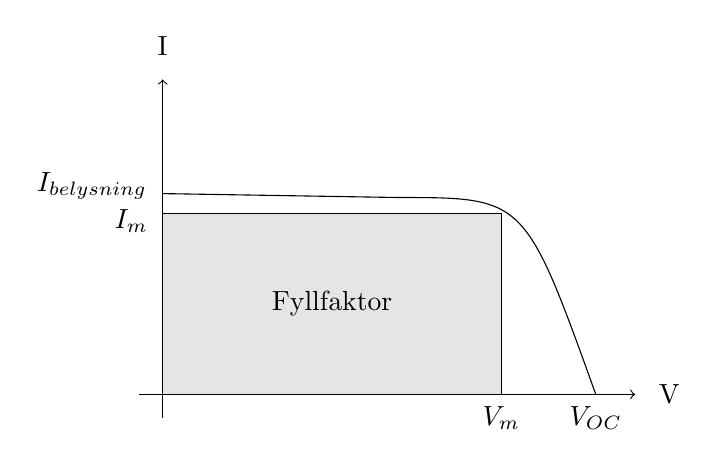
\begin{tikzpicture}

	\draw [->] (-0.3,0) -- (6,0) node [right=5pt]	{V};  % X-akse
	\draw [->] (0,-0.3) -- (0,4) node [above=5pt]	{I}; % Y-akse

	% Faktisk kurve
	\draw [-] (0,2.55) -- (3,2.5);
	\draw [-] (3,2.5) .. controls +(right:1.6cm) .. (5.5,0);
	
	% Fyllfaktor
	\node [draw, rectangle,fill=black!10,minimum height=2.3cm, minimum width=4.3cm] (FF) at (2.15,1.15) {Fyllfaktor};
	
	% Tekst
	\node at (-0.9,2.65) {$I_{belysning}$};
	\node at (-0.4,2.2) {$I_m$};
	\node at (4.3,-0.3) {$V_m$};
	\node at (5.5,-0.3) {$V_{OC}$};
	
	
\end{tikzpicture}

\caption{Str�m-spenningskarakterisitikken for en solcelle}%
\label{fig:fyllfaktor}%
\end{figure}



\bibliographystyle{plain}
\nocite{}

\bibliography{bibliography} % bibliography.bib


\end{document}

% Referanseliste

